Stokes problem is given by
\begin{equation}
    \begin{split}
        -\Delta u + \nabla p &= f \quad \text{in } \Omega, \\
        \nabla \cdot u &= 0 \quad \text{in } \Omega, \\
        u &= g \quad \text{on } \partial\Omega_D, \\
        \frac{\partial u}{\partial n} - p\, n &= h \quad \text{on } \partial\Omega_N. \\
    \end{split}
\end{equation}
Here, \( u \colon \Omega \to \mathbb{R}^n \) is the fluid field, while \( p \colon \Omega \to \mathbb{R} \) is the pressure field.
The presence of both the Dirichlet and Neumann boundary conditions leads to a well-posed problem, as long as neither is empty.
If we don't have a Dirichlet boundary, then the velocity field is only determined up to a constant, while if the Neumann boundary is empty, the pressure field is only determined up to a constant.

We find the weak form of the Stokes problem by multiplying the first equation by a test function \( v \in V \) and integrating.
This yields
\begin{align*}
    \int_{\Omega} \left(
        -\Delta u + \nabla p
    \right) \cdot v \diff x &= \int_{\Omega} f \cdot v \diff x, \\
    \int_{\Omega} \nabla u \cdot \nabla v \diff x - \int_\Omega p \nabla \cdot v \diff x &= \int_{\Omega} f \cdot v \diff x + \int_{\partial\Omega} \left(
        \frac{\partial u}{\partial n} - p\, n
    \right) \cdot v \diff s.
\end{align*}
Now applying the boundary conditions, we can split the boundary integral into two parts, one for the Dirichlet boundary and one for the Neumann boundary:
\begin{equation}
    \int_{\partial\Omega} \left(
        \frac{\partial u}{\partial n} - p\, n
    \right) \cdot v \diff s = \int_{\partial\Omega_D} \left(
        \frac{\partial u}{\partial n} - p\, n
    \right) \cdot v \diff s + \int_{\partial\Omega_N} \left(
        \frac{\partial u}{\partial n} - p\, n
    \right) \cdot v \diff s.
\end{equation}
As the solution is known on $\partial\Omega_D$, we can choose $v \in H^1_{0, D}(\Omega)$, such that the first term vanishes.
For the second term, we can simply insert the Neumann condition, which finally gives us
\begin{equation}
    \int_{\Omega} \nabla u \cdot \nabla v \diff x - \int_\Omega p \nabla \cdot v \diff x = \int_{\Omega} f \cdot v \diff x + \int_{\partial\Omega_N} h \cdot v \diff s.
\end{equation}
For the second equation, we multiply by a test function \( q \in Q \) and integrate, which gives us
\begin{equation}
    \int_{\Omega} q \nabla \cdot u \diff x = 0.
\end{equation}
The weak form of the problem is then to find \( (u, p) \in H_{g, D}^1(\Omega) \times L^2(\Omega) \) such that
\begin{equation}
    \begin{split}
        a(u, v) + b(p, v) &= f(v) \quad \forall v \in H_{0,D}^1(\Omega), \\
        b(q, u) &= 0 \:\,\qquad \forall q \in L^2(\Omega).
    \end{split}
\end{equation}
Note that we have here switched \( p := -p \), in order to get symmetry.

For saddle-point problems of the form described, the four Brezzi conditions we need to satisfy is then
\begin{enumerate}
    \item Continuity of $a$: For all \( u_h, v_h \in V_h \), we have
        \begin{equation}
            a(u_h, v_h) \leq C_1 \norm{u_h}_{V_h} \norm{v_h}_{V_h}.
        \end{equation}

    \item Coercivity of $a$: There exists a constant \( C_2 > 0 \) such that
        \begin{equation}
            a(u_h, u_h) \geq C_2 \norm{u_h}_{V_h}^2
        \end{equation}
        for all $u_h \in Z_h$, where
        \begin{equation*}
            Z_h = \{u_h \in V_h \mid b(u_h, q_h) = 0 \quad \forall q_h \in Q_h \}.
        \end{equation*}

    \item Continuity of $b$: For all \( q_h \in Q_h \) and \( u_h \in V_h \), we have
        \begin{equation}
            b(q_h, u_h) \leq C_3 \norm{q_h}_{Q_h} \norm{u_h}_{V_h}.
        \end{equation}

    \item ``Coercivity'' of $b$: There exists a constant \( C_4 > 0 \) such that
        \begin{equation}
            \sup_{u_h \in V_h}\, \frac{b(q_h, u_h)}{\norm{u_h}_{V_h}} \geq C_4 \norm{u_h}_1 \quad \forall q_h \in Q_h.
        \end{equation}
\end{enumerate}
For Stokes problem, the first three conditions aren't too difficult to check.
The last one however is a bit tricky, and typically requires specially designed finite elements in order to satisfy it.

Oscillations appear when the last condition is not satisfied.
This happens because there exists some $q_h \in Q_h$ such that $b(q_h, u_h) = 0$ for all $u_h \in V_h$, while $q_h \neq 0$.
This means that if we have some solution pressure $p_h \in Q_h$, we can simply add as much of $q_h$ as we want.
These spurious pressure modes typically take the form of oscillations.

For mixed elements, we get the expected approximation of
\begin{equation}
    \norm{u - u_h}_{1} + \norm{p - p_h}_{0} \leq C h^k \norm{u}_{k+1} + D h^{t+1} \norm{p}_{t+1},
\end{equation}
where $k$ is the polynomial degree of the velocity space and $t$ is the polynomial degree of the pressure space.

One popular choice of element is the Taylor--Hood element, % chktex 8
which is quadratic in velocity and linear in pressure, while being continuous across element boundaries.
In other words, it's a $P_2$-$P_1$ element.
This gives the expected approximation order of
\begin{equation}
    \norm{u - u_h}_{1} + \norm{p - p_h}_{0} \leq h^2 \left(
        C \norm{u}_{3} + D \norm{p}_{2}
    \right).
\end{equation}
Another popular choice is the mini element, which is linear in both velocity and pressure, however it has an additional bubble function in the velocity.
This bubble function is designed such that it is zero along the element edges, which on the unit triangle means that the basis functions are
\begin{equation}
    \{ 1, x, y, xy(1 - x - y) \},
\end{equation}
where the last function is the bubble function.
This gives the expected approximation order
\begin{equation}
    \norm{u - u_h}_{1} + \norm{p - p_h}_{0} \leq h \left(
        C \norm{u}_{2} + D h \norm{p}_{2}
    \right).
\end{equation}

Finally we have the Crouzeix--Raviart element, % chktex 8
which is linear in velocity and constant in pressure.
Additionally, the velocity is only continuous at the midpoint of each edge,
as illustrated in \cref{fig:crouzeix_raviart}.
With this element, we get the expected approximation order
\begin{equation}
    \norm{u - u_h}_{1} + \norm{p - p_h}_{0} \leq h \left(
        C \norm{u}_{2} + D \norm{p}_{1}
    \right).
\end{equation}

\begin{figure}[htbp]
    \centering
    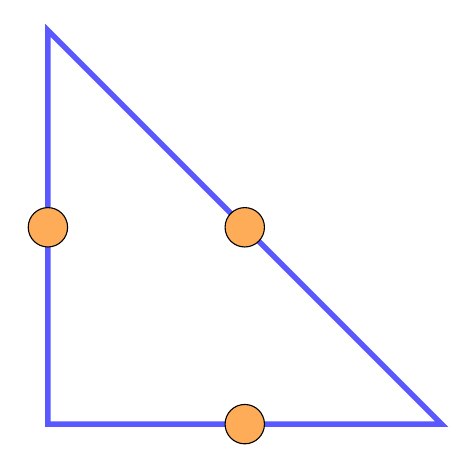
\begin{tikzpicture}[scale=5]
        \draw[line width=2, color=blue!65] (0, 0) -- (1, 0) -- (0, 1) -- cycle;
        \draw[fill=orange!65] (0.5, 0)   circle (0.05);
        \draw[fill=orange!65] (0,   0.5) circle (0.05);
        \draw[fill=orange!65] (0.5, 0.5) circle (0.05);
    \end{tikzpicture}
    \caption{
        Crouzeix--Raviart element with DOFs marked in orange.% chktex 8
        \label{fig:crouzeix_raviart}
    }
\end{figure}